% AtlasSAT-16U | Document 2A | Orbital Analysis One-Pager
% Style adapted from user-supplied 3B(2).tex, not its outdated simulation results.
\RequirePackage{fix-cm}
\documentclass[10pt,a4paper]{article}
\usepackage[a4paper,top=8mm,bottom=8mm,left=8mm,right=8mm]{geometry}
\usepackage[T1]{fontenc}

\usepackage{microtype,helvet}
\renewcommand{\familydefault}{\sfdefault}
\usepackage{xcolor,booktabs,tabularx,colortbl,mdframed,tikz,enumitem,hyperref,array,graphicx,multirow,amssymb}
\usetikzlibrary{shapes.geometric,arrows.meta,positioning,fit,backgrounds,calc}
\definecolor{atlasblue}{HTML}{0C447C}
\definecolor{atlasbluelight}{HTML}{185FA5}
\definecolor{atlasgray}{HTML}{444441}
\definecolor{atlaslightgray}{HTML}{F1EFE8}
\definecolor{atlasgreen}{HTML}{3B6D11}
\definecolor{passbg}{HTML}{EAF3DE}
\definecolor{passgreen}{HTML}{27500A}
\definecolor{todobg}{HTML}{FAEEDA}
\definecolor{todoorange}{HTML}{854F0B}
\definecolor{wippurple}{HTML}{EEEDFE}
\definecolor{wippurpletext}{HTML}{3C3489}
\definecolor{headerbg}{HTML}{E6F1FB}
\definecolor{rowalt}{HTML}{F8F8F6}
\setlength{\parindent}{0pt}\setlength{\parskip}{1.5pt}
\pagestyle{empty}
\hypersetup{colorlinks=true,linkcolor=atlasblue,urlcolor=atlasbluelight,pdftitle={AtlasSAT-16U Document 2A One-Page Orbital Analysis},pdfauthor={Wassim Ait Oubahou},pdfsubject={Public-distribution derivative RC v0.2; Document 2A RevD3.4; Codex-assisted preliminary mission analysis},pdfkeywords={AtlasSAT, GMAT, coverage, revisit, portfolio, RevD3.4}}
\newcommand{\colhead}[1]{{\fontsize{7.6}{10}\selectfont\bfseries\color{atlasblue}#1}\\[-3pt]\textcolor{atlasblue}{\rule{\linewidth}{0.4pt}}\vspace{1pt}}
\newcommand{\bhold}{\colorbox{todobg}{\textcolor{todoorange}{\textbf{\fontsize{5.5}{7}\selectfont\ NOT MET\ }}}}
\newcommand{\bpre}{\colorbox{wippurple}{\textcolor{wippurpletext}{\textbf{\fontsize{5.5}{7}\selectfont\ PRELIM.\ }}}}
\graphicspath{{../figures/}}
\newcommand{\bodyfont}{\fontsize{8.0}{11}\selectfont}
\renewcommand{\tabularxcolumn}[1]{>{\raggedright\arraybackslash}p{#1}}
\begin{document}
\begin{mdframed}[backgroundcolor=atlasblue,linewidth=0pt,innertopmargin=4pt,innerbottommargin=4pt,innerleftmargin=9pt,innerrightmargin=9pt]
\begin{minipage}[c]{0.56\linewidth}
{\fontsize{16}{19}\selectfont\bfseries\color{white}AtlasSAT-16U}%
\enspace{\fontsize{8.5}{11}\selectfont\color{white!65!atlasblue}Souss Water Observation CubeSat}\\[1pt]
{\fontsize{7}{9}\selectfont\color{white!55!atlasblue}Independent Research Project \textbar{} Document 2A \textbar{} Orbital Analysis \textbar{} Rev D3.4 \\ \href{mailto:wassim.aitoubahou@gmail.com}{\textcolor{white!65!atlasblue}{wassim.aitoubahou@gmail.com}}}
\end{minipage}\hfill
\begin{minipage}[c]{0.40\linewidth}\raggedleft
{\fontsize{7}{9.5}\selectfont\color{white!65!atlasblue}
16U CubeSat $\cdot$ 550 km near-SSO $\cdot$ GMAT R2026a\\
VNIR pushbroom $\cdot$ 30 km nominal swath\\
Chtouka-Massa agriculture, south of Agadir}
\end{minipage}
\end{mdframed}




\vspace{4pt}
\noindent\begin{minipage}[t]{.288\linewidth}\raggedright
\colhead{ENGINEERING OBJECTIVE}
{\bodyfont Test whether one AtlasSAT-16U can offer agricultural targets south of Agadir a \textbf{daylight opportunity every $\leq72$ h}. Preserved GMAT dynamics, provisional GIS targets and checked optical-access calculations form the evidence.\par}

\vspace{6pt}\colhead{PRESERVED CONCEPT}
{\fontsize{7.8}{10.3}\selectfont\setlength{\tabcolsep}{2pt}
\begin{tabularx}{\linewidth}{@{}lX@{}}\toprule\rowcolor{headerbg}Model & Adopted input\\\midrule
Orbit & Near-SSO, 550 km concept\\\rowcolor{rowalt}
Semimajor axis & 6928.1363 km\\
Ecc. / incl. & $e$=0.001; $i$=97.5$^\circ$\\\rowcolor{rowalt}
RAAN & 6.463$^\circ$\\
AOP / TA & 0$^\circ$ / 0$^\circ$ (canonical)\\\rowcolor{rowalt}
Epoch (UTC) & 20 Oct 2026,\newline12:00:00.000\\
Initial axes & EarthMeanOfDate\newline(Earth; MODEq)\\\rowcolor{rowalt}
LTDN / span & 10:30 mean solar; 30 days\\
Payload & Five-band VNIR pushbroom\\\rowcolor{rowalt}
Swath / roll & 30 km; nadir, ideal $\pm10^\circ$ and $\pm20^\circ$\\
Daylight & Target Sun elevation $\geq0^\circ$\\
\bottomrule\end{tabularx}}

\vspace{6pt}\colhead{WHAT WAS VERIFIED}
{\bodyfont Archived orbit benchmark: \textbf{36 numerical checks}. Coverage geometry: \textbf{570 opportunities at 31 targets}; maximum boundary difference \textbf{1.197 $\mu$s}. Numerical consistency is not physical accuracy.\par}

\vspace{6pt}\colhead{FOUR EVIDENCE LEVELS}
{\fontsize{7.8}{10.3}\selectfont
\textbf{Passage:} a track crosses the region.\\[3pt]
\textbf{Reachability:} a target lies inside an ideal sensor envelope.\\[3pt]
\textbf{Daylight opportunity:} reachability plus illumination.\\[3pt]
\textbf{Physical validation:} an achievable imaging service remains unproven.\par}

\vspace{6pt}\colhead{PRESERVED NEAR-SSO GEOMETRY}
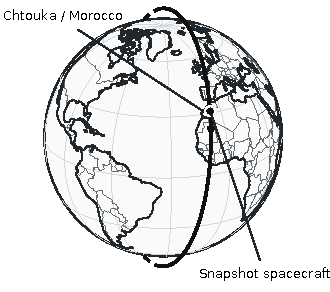
\includegraphics[width=\linewidth]{10_Orbital_Globe_Compact_RevD3_4.pdf}
{\fontsize{6.8}{8.5}\selectfont\color{atlasgray}1 Nov 2026, 11:23:49 UTC snapshot. True orbit-to-Earth scale; solid near-side / dashed far-side arc. Predicted orientation. Natural Earth context.\par}
\end{minipage}\hspace{2.4mm}%
\begin{minipage}[t]{.400\linewidth}\raggedright
\colhead{CHTOUKA--MASSA AGRICULTURAL TARGET}
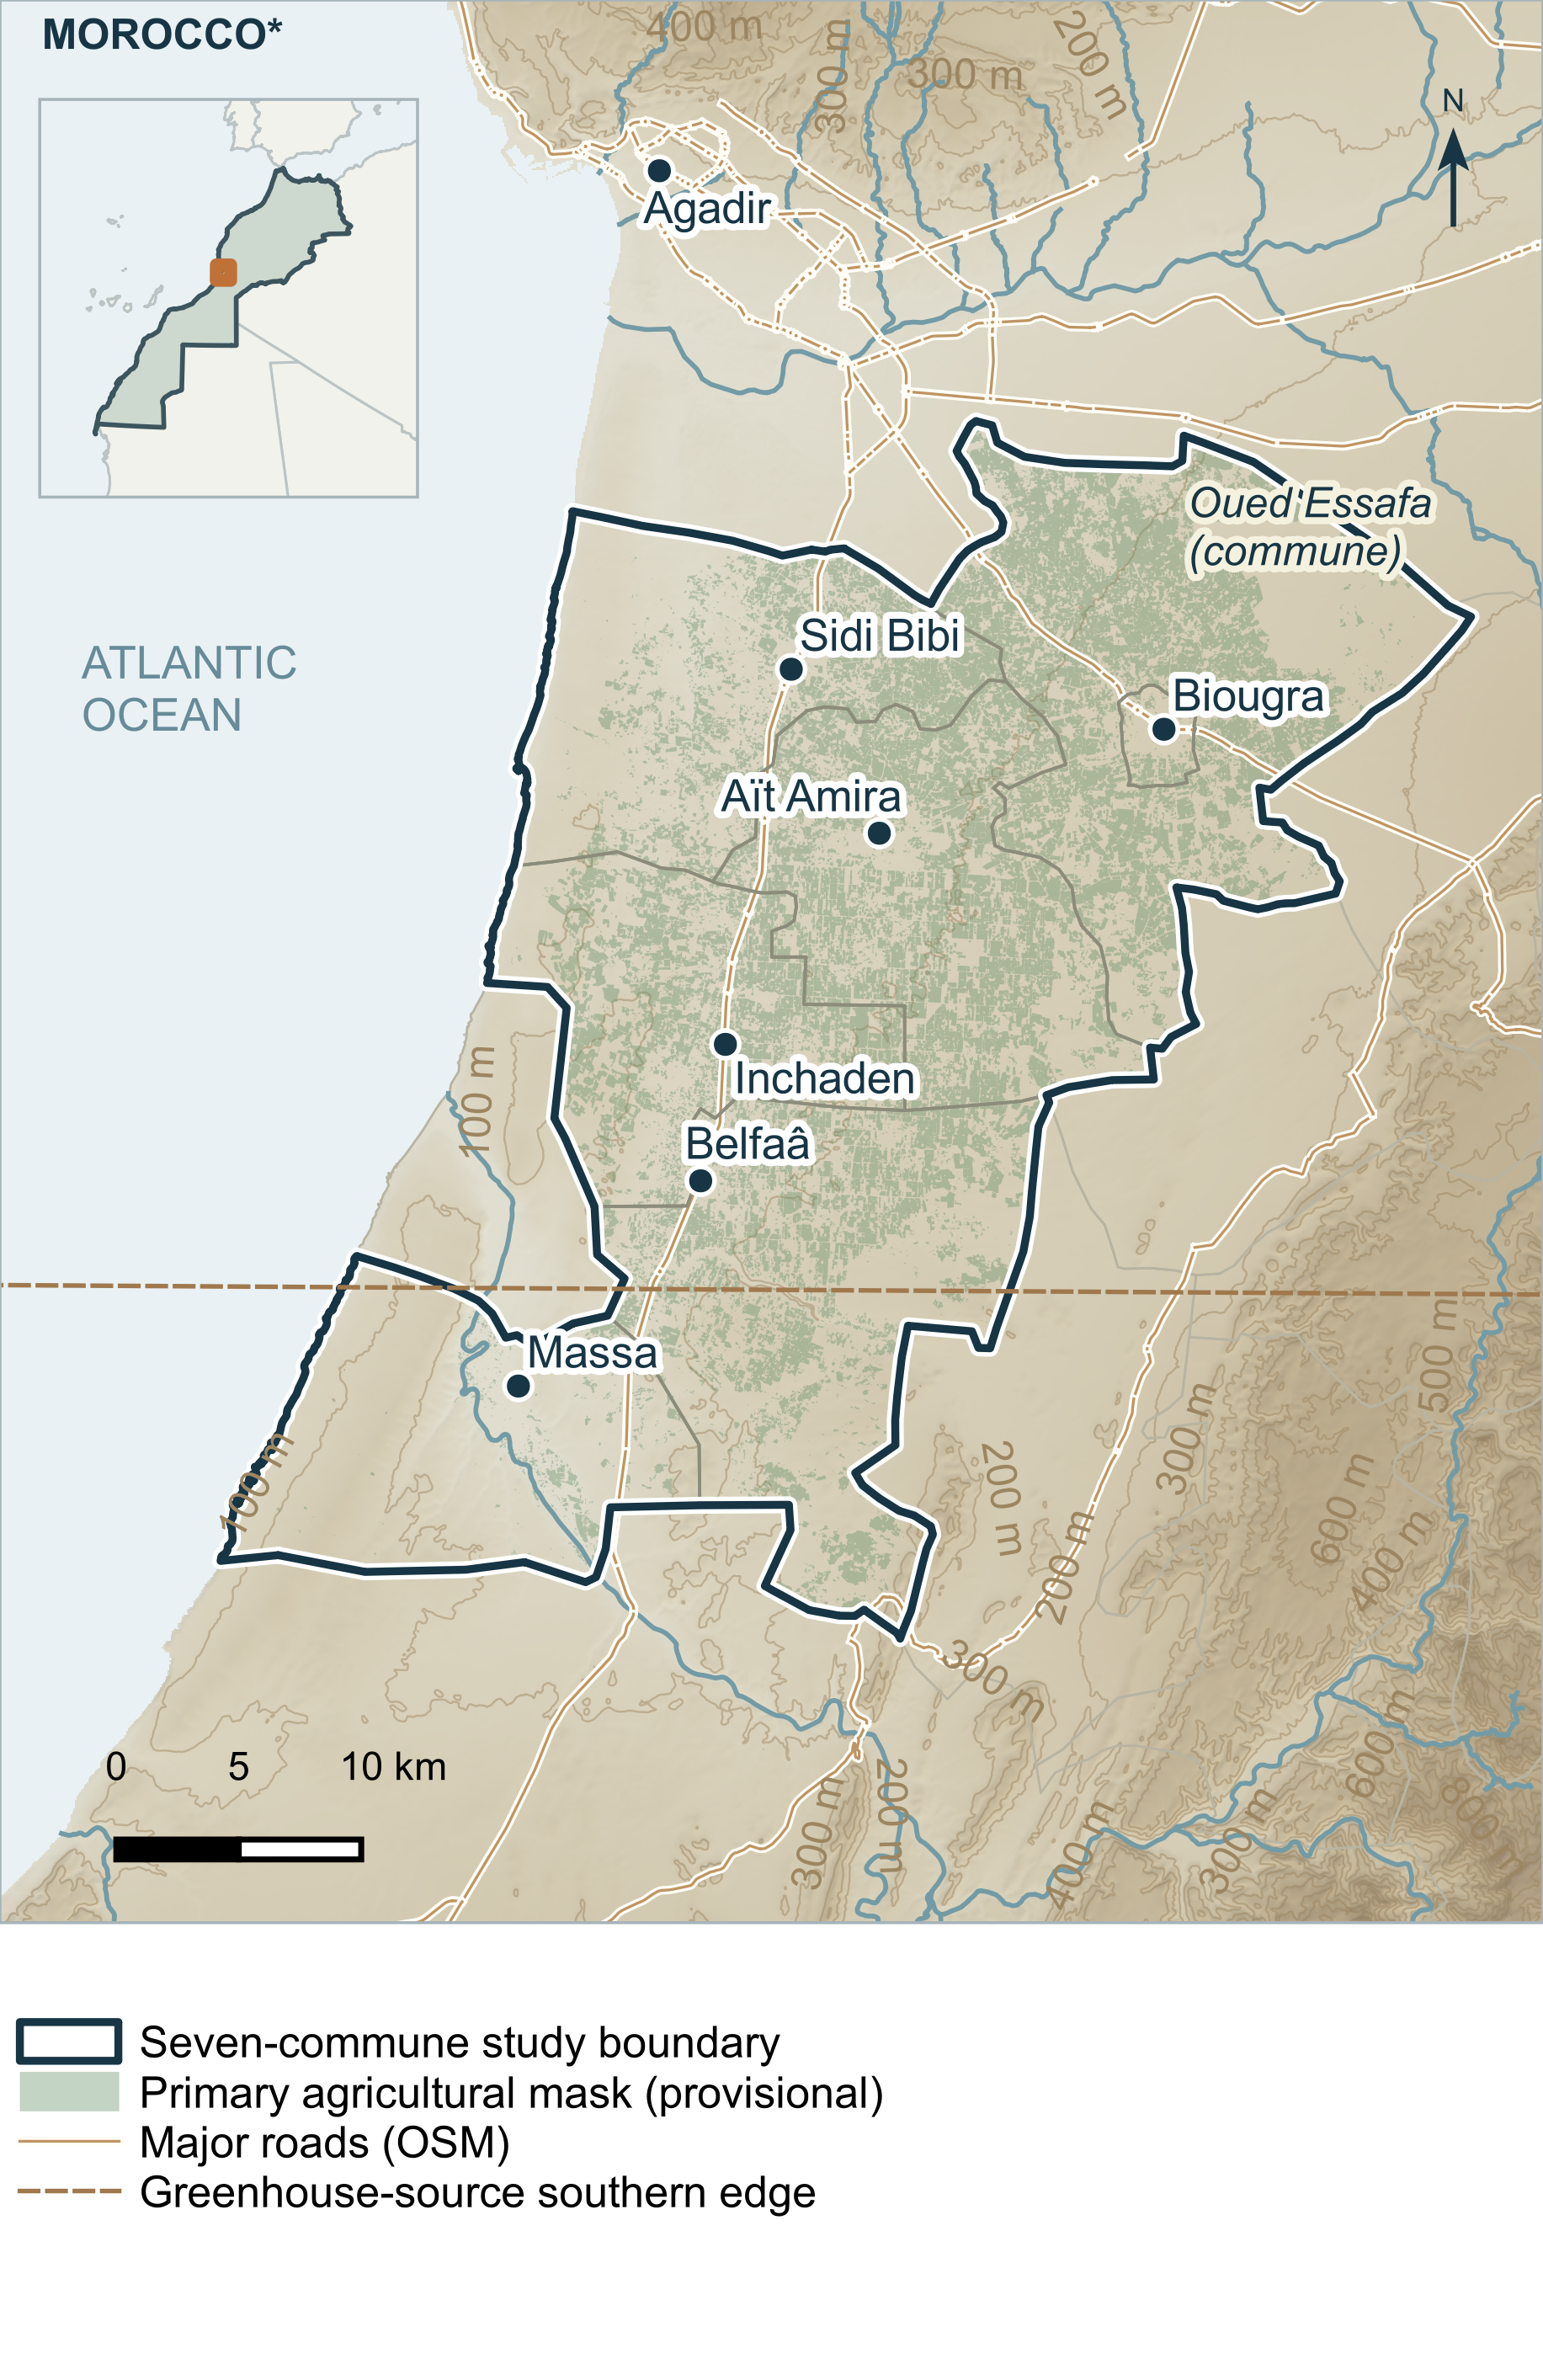
\includegraphics[width=\linewidth]{11_Technical_Atlas_Compact_RevD3_2.png}
{\fontsize{6.5}{8.0}\selectfont\color{atlasgray}*Morocco locator: geographic context only.\\WGS84 / UTM 29N; grid-north arrow.\par}
\vspace{3pt}
{\fontsize{7.6}{10.1}\selectfont\textbf{396.47 km$^2$} primary mask in a \textbf{1,173.92 km$^2$} seven-commune envelope. \textbf{Provisional research ROI}, not an official agricultural perimeter.\par}

\vspace{6pt}\colhead{KEY RESULTS \textbar{} DAYLIGHT \textbar{} 30 km}
{\fontsize{7.35}{9.7}\selectfont\setlength{\tabcolsep}{2pt}
\begin{tabularx}{\linewidth}{@{}Xrrr@{}}\toprule\rowcolor{headerbg}Metric & Nadir & $\pm10^\circ$ & $\pm20^\circ$\\\midrule
Mean 72 h area & 11.48\% & 22.76\% & 33.44\%\\\rowcolor{rowalt}
Max complete gap & 360.01 h & 360.01 h & \textbf{312.22 h}\\
Largest span* & 720 h & 360.01 h & 312.22 h\\\bottomrule\end{tabularx}}
{\fontsize{6.9}{8.6}\selectfont\color{atlasgray}*Includes endpoint censoring. Hourly window starts; 250 m area quadrature. Opportunities, not acquired images.\par}

\vspace{6pt}\colhead{ENGINEERING SIGNIFICANCE}
{\bodyfont Slow ground-track drift clusters opportunities rather than providing daily service. A favourable mean cannot replace a maximum-gap test; a night pass cannot meet daylight needs. The analytical note checks this interpretation; future design trades remain unperformed.\par}
\end{minipage}\hspace{2.4mm}%
\begin{minipage}[t]{.282\linewidth}\raggedright
\colhead{DAYLIGHT REVISIT VERDICT}
\begin{mdframed}[backgroundcolor=todobg,linecolor=todoorange,linewidth=.75pt,skipabove=2pt,skipbelow=2pt,innertopmargin=8pt,innerbottommargin=8pt,innerleftmargin=6pt,innerrightmargin=6pt]
\raggedright
{\fontsize{12}{14}\selectfont\bfseries\color{todoorange}NOT MET}\\[5pt]
{\fontsize{10}{12}\selectfont\textbf{312.22 h} vs \textbf{72 h}}\\[4pt]
{\bodyfont Longest complete gap with ideal $\pm20^\circ$ roll. All 14,494 samples fail the 72 h test.\par}
\end{mdframed}

\vspace{7pt}\colhead{30-DAY DAYLIGHT ACCESS TIMELINE}
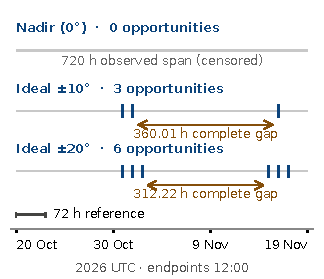
\includegraphics[width=\linewidth]{13_Daylight_Timeline_Compact.pdf}
{\fontsize{6.9}{8.7}\selectfont\color{atlasgray}30 km; Sun $\geq0^\circ$. Ticks: point opportunities, not acquired images or time-scaled bars. E16.\par}

\vspace{7pt}\colhead{TRACEABLE WORST CASE}
{\bodyfont Sidi Bibi target \texttt{sidi-bibi\_\allowbreak-10750\_\allowbreak19500}; 2--15 November. REF lies outside the ROI and is \textbf{excluded}. Full coordinates and UTC endpoints: 2A-1 / E16.\par}

\vspace{6pt}\colhead{BOUNDARIES OF THE EVIDENCE}
{\fontsize{7.6}{10.2}\selectfont\begin{itemize}[leftmargin=*,itemsep=2pt,topsep=1pt]
\item \textbf{Provisional} agriculture; local classification accuracy unestablished.
\item Greenhouse-source gap: \textbf{22.04\%} of envelope / \textbf{6.861\%} of mask. Missing acreage unknown.
\item \textbf{Predicted} Earth orientation; preliminary forces.
\item Ideal roll is not qualified slew, pointing or image quality; physical/operational acquisition unvalidated.
\item TA90 changes initial TA at fixed osculating inputs, not phase alone at fixed mean orbit.
\end{itemize}\par}

\vspace{7pt}\colhead{NEXT STEPS}
{\fontsize{7.6}{10.1}\selectfont Next: phased 2--5 satellite constellation trades, followed by orbit-design, drag, solar-elevation and observation-scheduling studies.\par}

\vspace{7pt}\colhead{DETAILED ENGINEERING RECORD}
{\fontsize{7.6}{10.1}\selectfont\href{./AtlasSAT_2A-1_Orbital_Analysis_RevD3_5_Public_RC_v0_2.pdf}{\textbf{2A-1, Rev D3.4}}: methods and gap provenance. E15: native GUI-first script (bundled). Codex-assisted implementation; detailed contribution note supplied.\par}
\end{minipage}
\vfill
{\fontsize{6.3}{8}\selectfont\color{atlasgray}\copyright\ ESA WorldCover project 2021 / Contains modified Copernicus Sentinel data (2021) processed by ESA WorldCover consortium.\\\copyright\ OpenStreetMap contributors: \url{https://www.openstreetmap.org/copyright}. \href{https://doi.org/10.5281/zenodo.7875105}{WorldCereal 2021 (Van Tricht et al.)}; \href{https://doi.org/10.6084/m9.figshare.27731148.v2}{Global-PCG-10 (Niu et al.)}; \href{https://creativecommons.org/licenses/by/4.0/}{CC BY 4.0}.\\The organisations in charge of the Copernicus programme by law or by delegation do not incur any liability for any use of the Copernicus WorldDEM-30.\par}

{\fontsize{6.3}{8}\selectfont\color{atlasgray}\textbf{Preliminary research demonstrator \textbar{} Rev D3.4 \textbar{} 26 October 2026.} The inherited v0.2 integrity exception is disclosed in 2A-1; v0.3/v0.4 coverage is unchanged. GSD, optical IFOV and line rate remain separate, unvalidated quantities.\par
Relief produced using Copernicus WorldDEM-30 \copyright\ DLR e.V. 2010--2014 and \copyright\ Airbus Defence and Space GmbH 2014--2018, provided under COPERNICUS by the European Union and ESA; all rights reserved. OSM contributors (ODbL); ESA/PCG (CC BY); Natural Earth (public domain). Contains modified Copernicus Sentinel data (2026).\par}
\end{document}
